\documentclass[aspectratio=169]{beamer}

\author{С.Б. Лопес Висенс, В.В. Писарев\\
\small{Московский физико-технический институт (национальный исследовательский университет)} }
\title{Моделирование фильтрации двухкомпонентной смеси жидкости и идеального газа}
\date{29-11-2021}

% \usetheme{Copenhagen}
% \usecolortheme{beaver}
\usetheme{Montpellier}
\usecolortheme{spruce}

%gets rid of bottom navigation bars
\setbeamertemplate{footline}[frame number]{}

%gets rid of bottom navigation symbols
\setbeamertemplate{navigation symbols}{}

%gets rid of footer
%will override 'frame number' instruction above
%comment out to revert to previous/default definitions
\setbeamertemplate{footline}{}


\usepackage{graphicx}
\usepackage{float}
\usepackage[utf8]{inputenc}
\usepackage[T2A]{fontenc}
\usepackage{textcomp}
\usepackage{amsmath, amssymb}
\usepackage{siunitx}
\usepackage{xcolor}
\usepackage{bm}
\usepackage{cancel}
\usepackage{hyperref}

\AtBeginSection[]
{
    \begin{frame}
        \frametitle{План}
        \tableofcontents[currentsection]
    \end{frame}
}

\begin{document}
\maketitle
\Large

\section{Введение}

\begin{frame}
    \frametitle{Течение через пористую среду}

    \begin{columns}
    \begin{column}{0.6\textwidth}
        \begin{figure}[H]
            \centering
            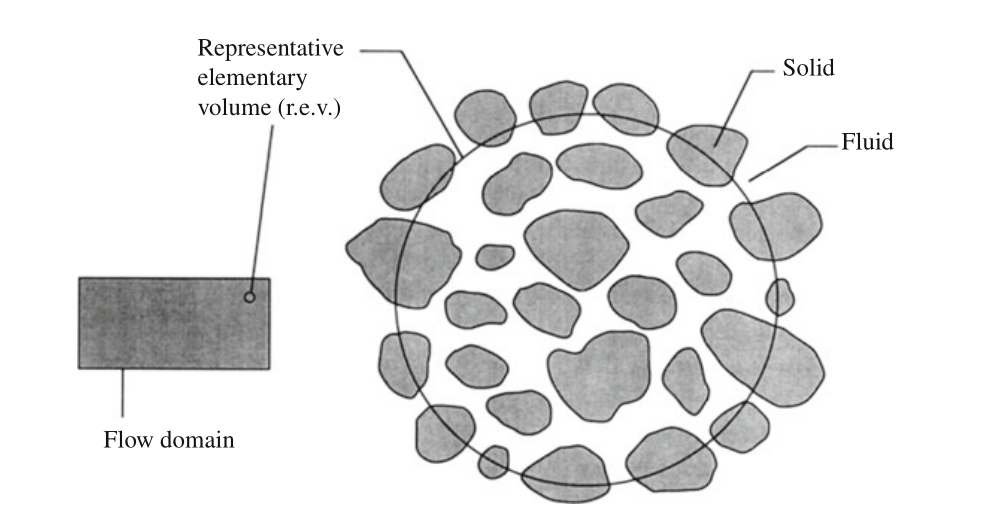
\includegraphics[width=\textwidth]
            {img/porous-medium.png}
        \end{figure}
    \end{column}
    \begin{column}{0.4\textwidth}
            Макроскопические уравнения течения получаются
            усреднением обычных уравнений по объёмам,
            содерживающим много пор.
    \end{column}
    \end{columns}

\end{frame}

\begin{frame}
    \frametitle{Скорость фильтрации и уравнения непрерывности}
    Скорость фильтрации - средняя скорость жидкости в свободном
    пространстве внутри пор.
    \[
    \vec v = \varphi \vec V_f
    \] 
    где \(\varphi\) - пористость среды, 
    \(\vec V_f\) - средняя скорость течения через объем, не
    содержащий поров.

    \begin{block}{Уравнеие непрерывности для каждого компонента}
        \begin{equation}
            \varphi \frac{\partial \rho_i}{\partial t}
            + div (\rho_i \bm{v}_i) = 0
        \end{equation}
    \end{block}
\end{frame}

\begin{frame}
    \frametitle{Закон Дарси: проницаемость}
    \begin{columns}
    \begin{column}{0.6\textwidth}
        \begin{block}{Закон Дарси для каждого компонента}
            \begin{equation}
                \mathbf{v}_i = -\frac{1}{\mu_i} K \cdot f_i (s)
                \cdot \nabla P
            \end{equation}
        \end{block}
        \(K\) --- коэффициент проницаемости,

        \(f\) --- относительная фазовая проницаемость,

        \(\mu\) --- динамическая вязкость,

        \(s\) --- газонасыщенность.
    \end{column}
    \begin{column}{0.4\textwidth}
        \begin{figure}[H]
            \centering
            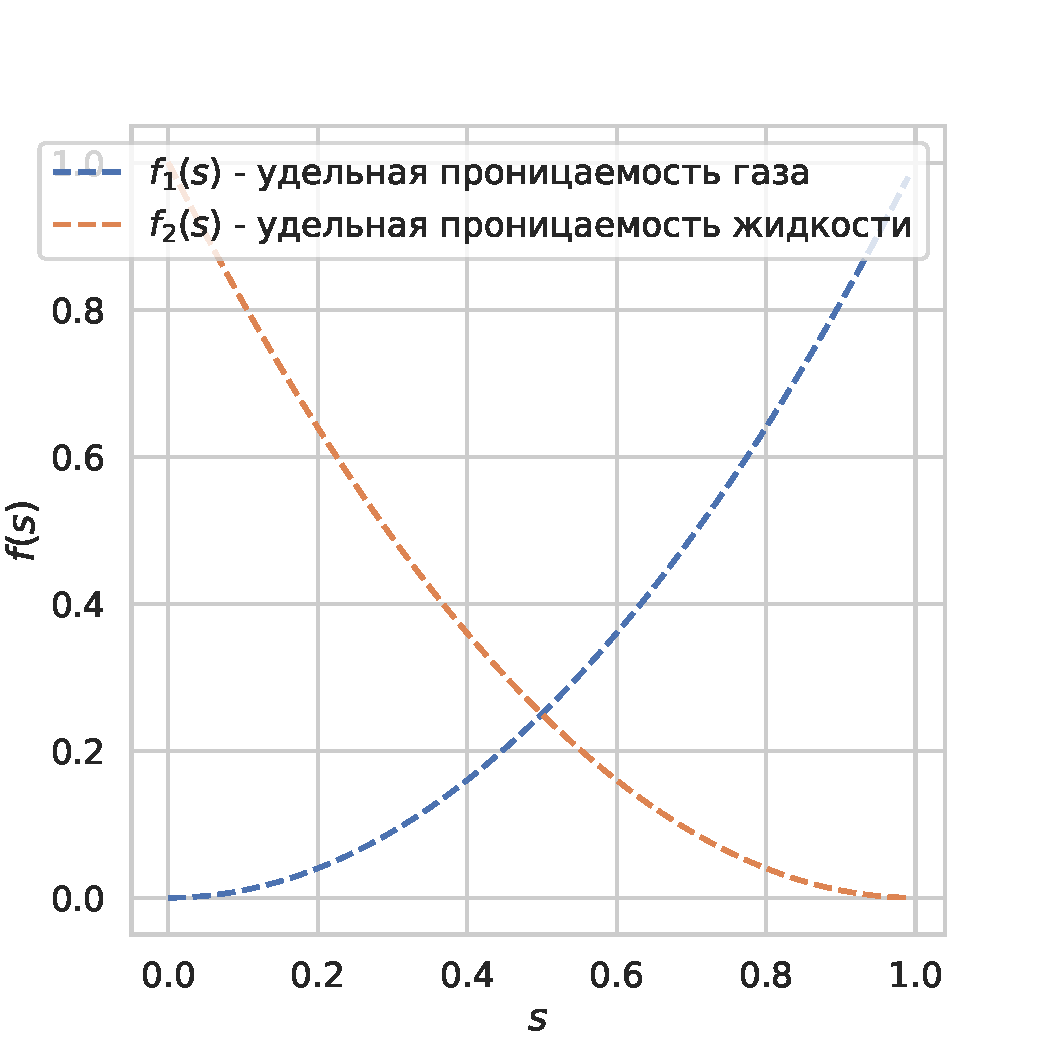
\includegraphics[width=\textwidth]{img/two-phase.pdf}
            \label{fig:}
        \end{figure}
    \end{column}
    \end{columns}
\end{frame}

\section{Постановка задачи}

\begin{frame}
    \frametitle{Постановка задачи}

    \begin{columns}

    \begin{column}{0.7\textwidth}
        \begin{figure}[H]
            \centering
            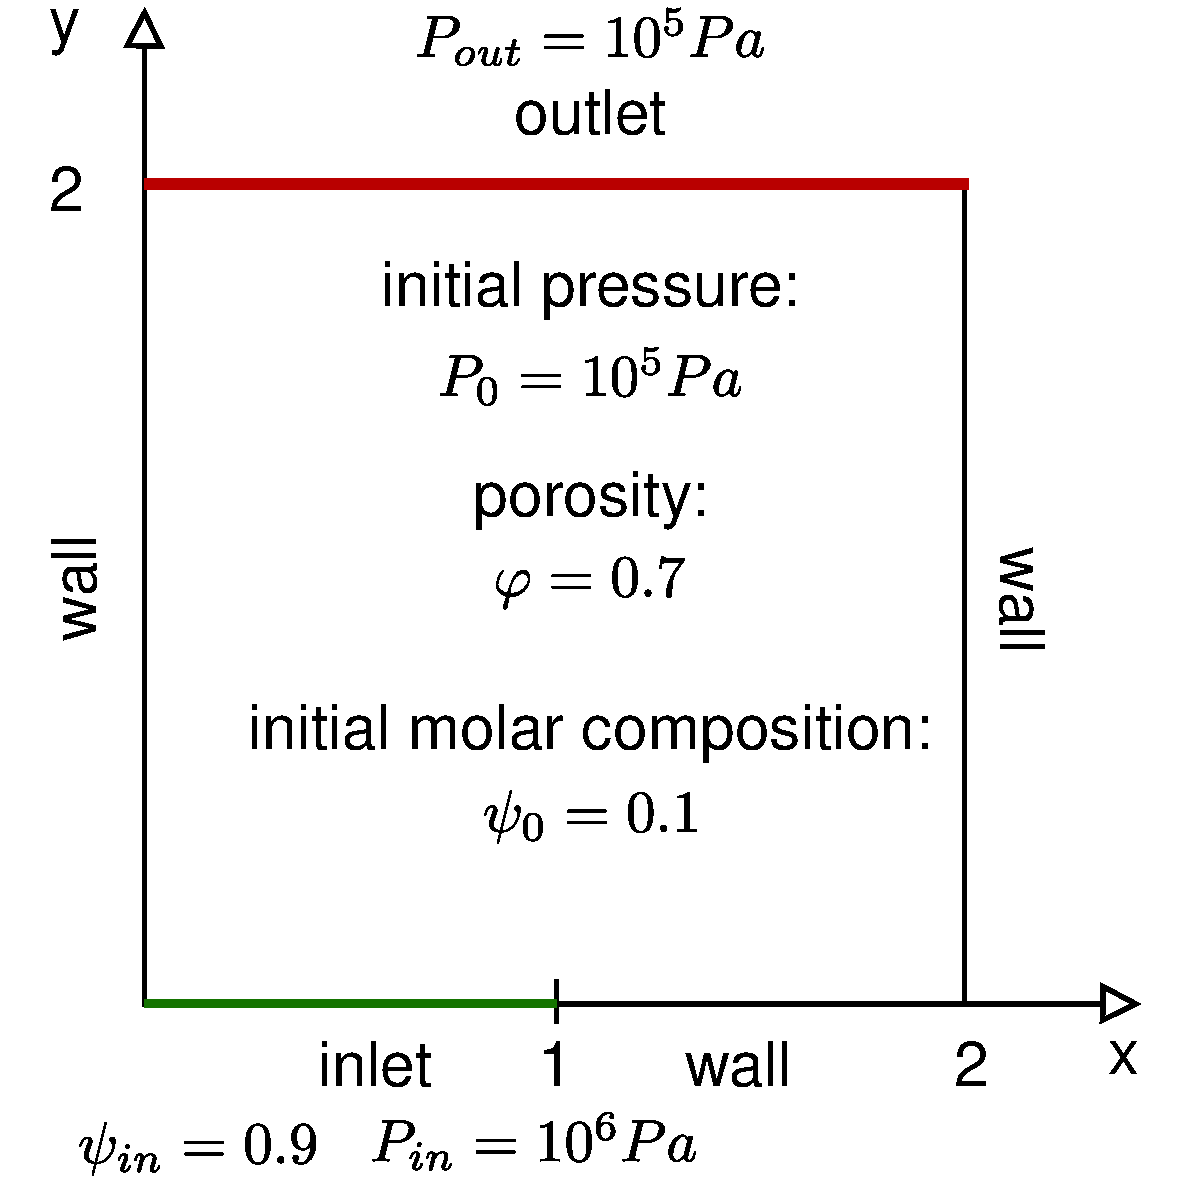
\includegraphics[height=0.8\textheight]
            {img/problem.pdf}
        \end{figure}
    \end{column}

    \begin{column}{0.4\textwidth}
        2-мерная задача:
        Моделирование фильтрации двухкомпонентной смеси 
        азота и пентана при предположении, что компоненты
        не смешиваются.
        Изотермическая задача.
    \end{column}

    \end{columns}

\end{frame}

% \input{goals.tex}
\section{Методы, применяемые в работе}
\begin{frame}
    \frametitle{Уравнения состояния}

    \begin{block}[Уравнеие Тейта для жидкости]
         \begin{equation}
             \frac{\hat{\rho} - \rho_0}{\hat{\rho}} = C \log_{10}
             \frac{B + P}{B + P_0}
         \end{equation}
    \end{block}
    \begin{block}[Уравнение идеального газа]
\begin{equation}
    P = \frac{RT}{M} \hat{\rho}
\end{equation}
    \end{block}

\end{frame}

\begin{frame}
    \frametitle{Методы, применяемые в работе}
        \begin{enumerate}
            \begin{columns}
            \begin{column}{0.6\textwidth}
                \item Метод конечных разностей второго порядка для
                    дискретизации по пространству с использованием
                    шахматной сеткой.
                \item Явный метод предиктор-корректор по схеме Хойна
                    для интегрирования по времени.
            \end{column}
            \begin{column}{0.4\textwidth}
                \begin{figure}[H]
                    \centering
                    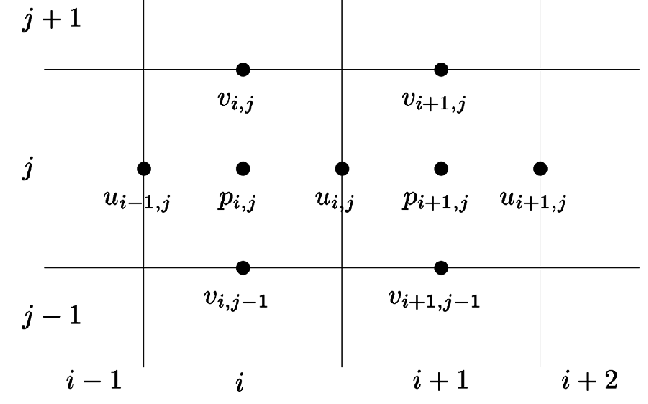
\includegraphics[width=\textwidth]
                    {img/staggered-grid.png}
                \end{figure}
            \end{column}
            \end{columns}
            \item Метод Ньютона-Рафсона для нахождения
                давления и газонасыщенности.
        \end{enumerate}
\end{frame}

\section{Основная часть}

\begin{frame}
    \frametitle{Алгоритм}
    \begin{enumerate}
        \item Вычисление плотностей при помощи уравнений состояния.
        \item Нахождение давления и газонасыщенности методом
            Ньютона-Рафсона из условия равенства давления газа
            и жидкости.
        \item Вычисление скоростей законом Дарси.
        \item Переход на следующий шаг по времени согласно
            численной схеме.
    \end{enumerate}

\end{frame}

\begin{frame}
    \frametitle{Результаты}
     \begin{figure}[H]
         \centering
         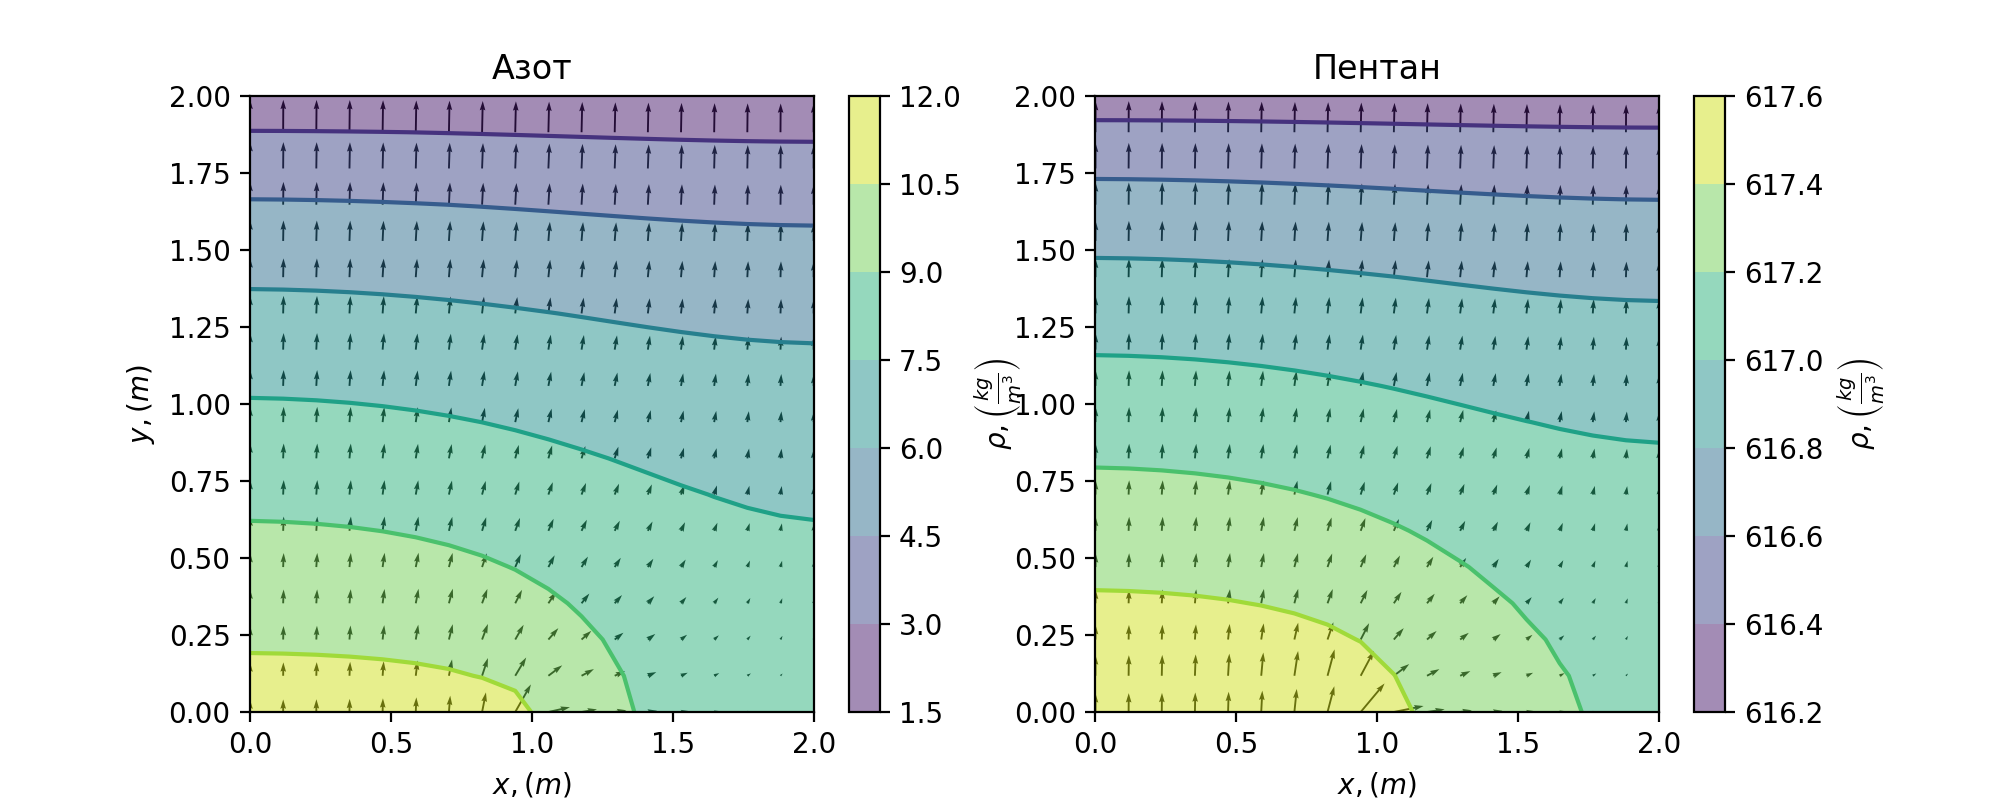
\includegraphics[width=\textwidth]
         {img/2phase-filtration-density.png}
     \end{figure}
\end{frame}

\begin{frame}
    \frametitle{Результаты}
     \begin{figure}[H]
         \centering
         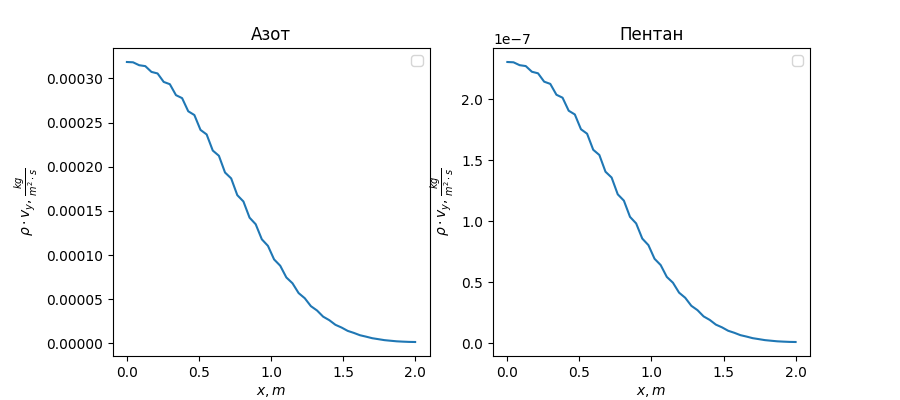
\includegraphics[width=0.9\textwidth]
         {img/flux.png}
     \end{figure}
\end{frame}

\section{Выводы}

\begin{frame}
Для указанных начальных и граничных условий решается
задача вытеснения смеси газа и жидкости обогащенной по газу
смесью с большой газонасыщенностью.
\end{frame}


\end{document}

